\documentclass[11pt,a4paper]{article}
\usepackage[utf8]{inputenc}
\usepackage[T1]{fontenc}
\usepackage[margin=1in]{geometry}
\usepackage{graphicx}
\usepackage{xcolor}
\usepackage{float}
\usepackage{listings}
\usepackage{upquote}
\usepackage{tcolorbox}

\lstset{
    basicstyle=\ttfamily\small,
    breaklines=true,
    frame=single,
    numbers=left,
    numberstyle=\tiny,
    backgroundcolor=\color{gray!10},
    keywordstyle=\color{blue},
    commentstyle=\color{green!50!black},
    stringstyle=\color{red},
    showstringspaces=false
}

\newtcolorbox{notebox}{colback=blue!5,colframe=blue!40!black,title=Note,fonttitle=\bfseries}

\title{\textbf{Practice 5 -- LiDAR Obstacle Avoidance}}
\author{
    Robotics and Cyber-Physical Systems \\
    School of Sciences and Engineering \\
    Tecnol\'ogico de Monterrey
}
\date{}

\begin{document}

\maketitle

\section*{Introduction}

In this activity, you will use the robot's 2D LiDAR to visualize nearby
objects and add simple obstacle avoidance to manual control. The same scripts
work with the physical robot and the MuJoCo simulator.

\subsection*{Before You Begin}

Update the repository and its dependencies:

\begin{lstlisting}[language=bash]
git pull
uv sync
\end{lstlisting}

Make sure the robot has enough clear space to move safely.

\section*{Part 1 -- Explore the LiDAR}

Run the existing demo:

\begin{lstlisting}[language=bash]
uv run examples/lidar_plot.py
\end{lstlisting}

Drive the robot slowly and observe how the points change. Each LiDAR reading
contains an angle and a distance. The plot converts these polar measurements
to Cartesian coordinates, with $+x$ pointing forward from the robot and $y$
pointing sideways.

\begin{figure}[H]
    \centering
    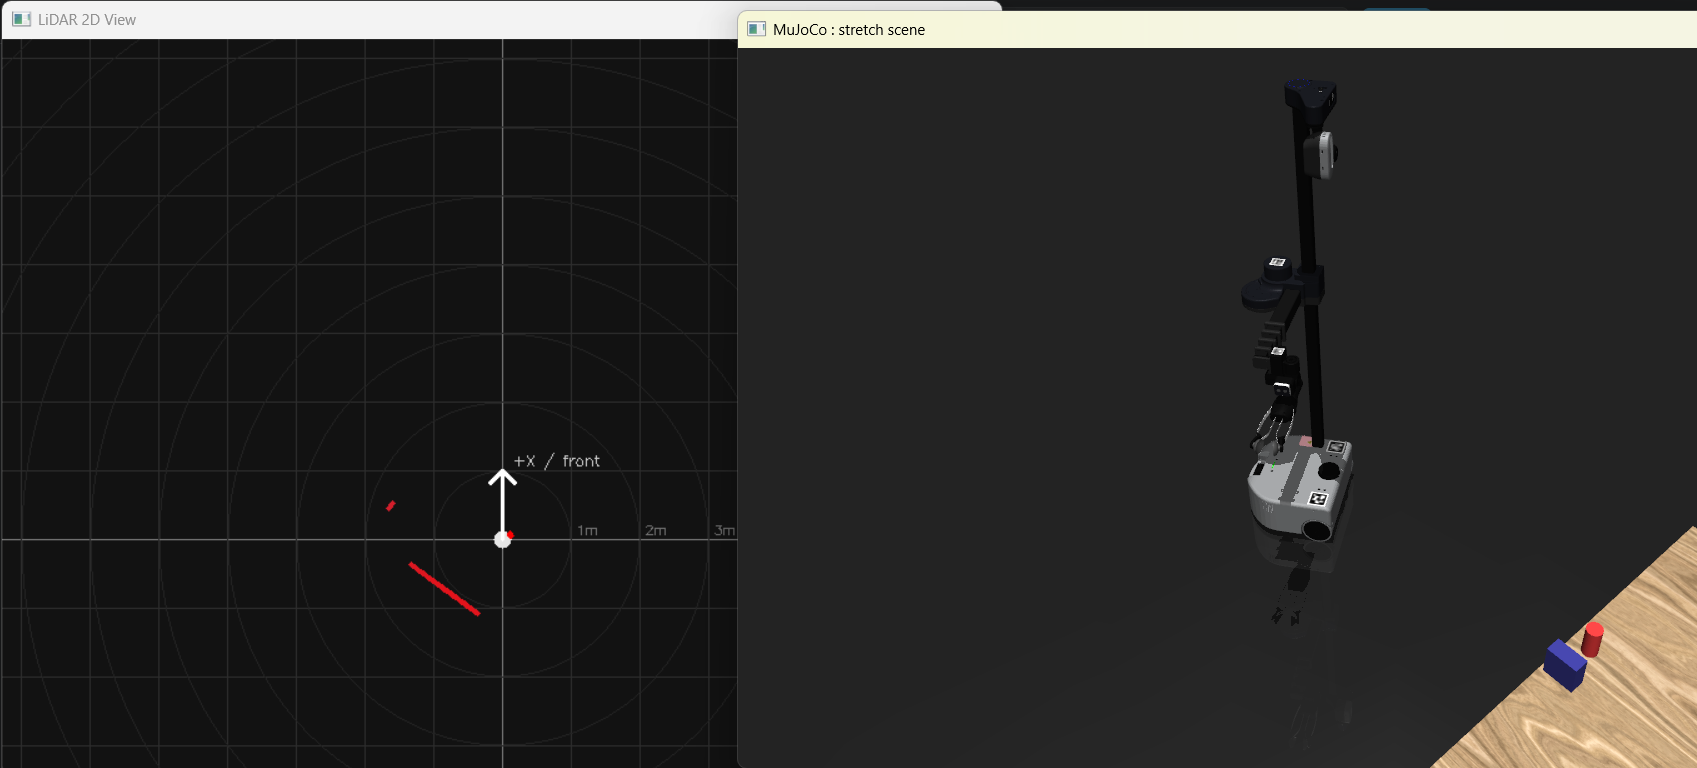
\includegraphics[width=0.72\textwidth]{lidar_demo.png}
    \caption{Top-down visualization of a LiDAR scan.}
\end{figure}

\section*{Part 2 -- Add Obstacle Avoidance}

Create a new script from the LiDAR demo:

\begin{lstlisting}[language=bash]
cp examples/lidar_plot.py lidar_obstacle_detection.py
\end{lstlisting}

\subsection*{1. Add the Imports and Constants}

Add NumPy, the mast filter, and the command-merging helper:

\begin{lstlisting}[language=Python]
import numpy as np

from stretch_tools import filter_mast_points
from stretch_tools.norm_vel_ctrl import merge_proportional

HALF_BASE_WIDTH = 0.175
FRONT_DETECTION_DISTANCE = 0.3
REAR_DETECTION_DISTANCE = 0.55
REAR_FULL_AVOIDANCE_DISTANCE = 0.15
\end{lstlisting}

The base is approximately 35 cm wide, so only points within $\pm 0.175$ m of
its centerline can block its path. The front and rear distances define how
early the avoidance response begins.

\subsection*{2. Calculate the Avoidance Command}

Add this function before \texttt{main()}:

\begin{lstlisting}[language=Python]
def get_obstacle_avoidance(scan):
    angles = np.radians([angle for _, angle, _ in scan])
    distances = np.array([distance for _, _, distance in scan]) / 1000
    x = distances * np.cos(angles)
    y = distances * np.sin(angles)

    front_obstacles = (
        (np.abs(y) <= HALF_BASE_WIDTH)
        & (x > 0)
        & (x <= FRONT_DETECTION_DISTANCE)
    )
    rear_obstacles = (
        (np.abs(y) <= HALF_BASE_WIDTH)
        & (x <= 0)
        & (x >= -REAR_DETECTION_DISTANCE)
    )

    contributions = []
    if front_obstacles.any():
        index = np.flatnonzero(front_obstacles)[np.argmin(x[front_obstacles])]
        contributions.append(-(1 - x[index] / FRONT_DETECTION_DISTANCE))

    if rear_obstacles.any():
        index = np.flatnonzero(rear_obstacles)[np.argmax(x[rear_obstacles])]
        closest = abs(x[index])
        authority = (REAR_DETECTION_DISTANCE - closest) / (
            REAR_DETECTION_DISTANCE - REAR_FULL_AVOIDANCE_DISTANCE
        )
        contributions.append(min(1.0, authority))

    if not contributions:
        return {}

    return {"base_forward": max(contributions, key=abs)}
\end{lstlisting}

A front obstacle contributes negative velocity, pushing the robot backward.
A rear obstacle contributes positive velocity. The contribution grows as the
obstacle gets closer, and the strongest response is used if both regions
contain points.

\subsection*{3. Combine Avoidance with Teleoperation}

Replace the body of the LiDAR loop with:

\begin{lstlisting}[language=Python]
for scan in lidar.iter_scans():
    scan = filter_mast_points(scan)
    avoidance = get_obstacle_avoidance(scan)
    teleop_command = teleop.get_normalized_velocities()
    command = merge_proportional(avoidance, teleop_command)

    controller.set_command(command)
    plotter.update(scan)
\end{lstlisting}

\texttt{merge\_proportional()} gives priority to its first dictionary. By
placing avoidance first, nearby obstacles progressively suppress an unsafe
manual command while the operator retains control of every other joint.

\begin{notebox}
Test at low speed. Approach an obstacle from the front and rear while watching
the LiDAR plot. Keep a hand ready to stop the robot during the first test.
\end{notebox}

\section*{Expected Result}

The robot should remain manually controllable. When an obstacle enters the
front corridor, forward motion should weaken and eventually reverse. The same
should happen in the opposite direction when backing toward an obstacle.

\end{document}
